\begin{frame}{Vigencias Futuras para Inversión (\% del PIB)}
\begin{figure}[h!]
    \centering
    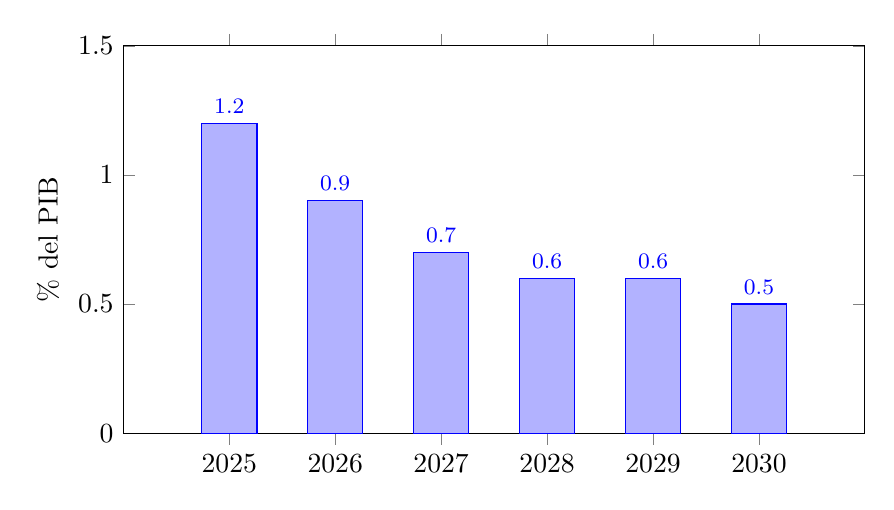
\begin{tikzpicture}
        \begin{axis}[
            ybar,
            bar width=20pt,
            ymin=0,
            ymax=1.5,
            ylabel={\% del PIB},
            symbolic x coords={2025, 2026, 2027, 2028, 2029, 2030},
            xtick=data,
            nodes near coords,
            nodes near coords style={font=\footnotesize},
            width=11cm,
            height=6.5cm,
            enlarge x limits=0.2,
            every axis plot/.append style={fill=gray!50}
        ]
            \addplot coordinates {
                (2025,1.2) (2026,0.9) (2027,0.7)
                (2028,0.6) (2029,0.6) (2030,0.5)
            };
        \end{axis}
    \end{tikzpicture}
    \vspace{0.3cm}
    \par\footnotesize{\textit{Fuente: Elaboración propia con base en MFMP 2024, MHCP.}}
\end{figure}
\end{frame}
